\documentclass[12pt]{report}
\usepackage
{
	multicol,
	hyperref,
	setspace,
	authblk,
	fancyhdr,
	graphicx,
	amsmath,
	filecontents
}
\usepackage[numbered,framed]{matlab-prettifier}
\lstMakeShortInline"

\lstset{
  style = Matlab-editor,
  basicstyle = \mlttfamily,
  escapechar = ",
  mlshowsectionrules = true,
}
\begin{filecontents*}{scaledata.m}
%   read in gaze data for subject
    data = dlmread(strcat(homepath,'/Working Directory/Data/',group,int2str(subject),'videoGZD.txt'),'	',15, 0);
%   select data relevant to the clip
    data = data(data(:,1)>(timestmps(1,clipno)*1000),:);
    data = data(data(:,1)<(timestmps(2,clipno)*1000),:);
    if clipno > 6
        data(:,3) = data(:,3) * 720/1280;
        data(:,10) = data(:,10) * 720/1280;
        data(:,4) = data(:,4) * 368/1024;
        data(:,11) = data(:,11) * 368/1024;
    else
        data(:,4) = data(:,4) * 720/1024;
        data(:,11) = data(:,11) * 720/1024;
    end
\end{filecontents*}

\begin{filecontents*}{overlay.m}
%   for each frame in the video
    while hasFrame(rdr)
        vidframe = readFrame(rdr);
        imshow(vidframe);
        hold on;
%       get the corresponding frame in the eye tracking data
        gzframe = data(i,:);
%       for every frame after the first
        if size(prevframe,1) > 0
%           plot the trace from the last left,right and centre gazepoints
%           to the current ones
            plot([prevframe(3) gzframe(3)],[prevframe(4) gzframe(4)],'b-');
            plot([prevframe(10) gzframe(10)],[prevframe(11) gzframe(11)],'r-');
            plot([prev_mn(1) mn_pnt(1)],[prev_mn(2) mn_pnt(2)],'k-');
        end
%       plot the current gazepoints on top of the trace to emphasise where
%       the gaze is travelling
        plot(gzframe(3),gzframe(4),'bx');
        plot(gzframe(10),gzframe(11),'rx');
        mn_pnt = mean([gzframe(3) gzframe(4);gzframe(10) gzframe(11)],1);
        plot(mn_pnt(1),mn_pnt(2),'kx','MarkerSize',10);
%       write the frame to the tracking video
        writeVideo(wrtr, getframe(gcf));
        prevframe = gzframe;
        prev_mn = mn_pnt;
        i = i + 1
    end
\end{filecontents*}

\begin{filecontents*}{elbowmethod.m}
        if ~exist('mix','var');
%         create mixture model, covariance set to full
            mix = gmm(2,num_centres, 'diag');

%         set options struct to use for dispExperting error at each cycle later
            mix = gmminit(mix,X,options);
        end

%     iterate through EM algorithm to improve fit to data points
        for i = 1:2000
            [mix, options] = gmmem(mix, X, options);
        end
	
        if num_centres ~= 1
            if options(8) - err > 1
                return;
            end 
        end
\end{filecontents*}

\begin{filecontents*}{singleft.m}
%   Sort features based on their individual classification accuracy
    y = [ones(8,1);zeros(7,1)-1];
    fn = @(XT, yT, Xt, yt)(sum(yt~=(predict(fitcsvm(XT, yT),Xt))));
    acc = zeros(1,size(X,2));
    
    for i = 1:size(X,2)
        ft = X(:,i);
%       Iterate through the partition objects test data and evaluate the
%       feature based on mean classification loss
        ftmdl = fitcsvm(ft,y,'KernelFunction','polynomial', 'KernelScale', 'auto','BoxConstraint',0.01);
        cvmdl = crossval(ftmdl, 'holdout', 0.3);
        acc(i) = 1 - kfoldLoss(cvmdl);
    end
    [val ind] = max(acc)
    cX = [acc;X];
    cX = sort(cX,2,'descend');
    cX = cX(2:end,:);
\end{filecontents*}

\setcounter{tocdepth}{2}
\begin{document}
	\begin{titlepage}
		\vspace*{\fill}
		\begin{center}
			
\includegraphics[width=3cm]{cardiffuni.png}\\[1cm]
			\Huge{Can we detect expert and novice anaesthetists by how they watch video?}\\[0.5cm]
			\Large{Liam Hiley - C1435690}\\[0.5cm]
			School of Computer Science and Informatics
		\end{center}
		\thispagestyle{fancy}
		\vspace*{\fill}
	\end{titlepage}
	\newpage
	\addtocontents{toc}{\protect\setcounter{tocdepth}{0}}
	\section*{Abstract}
		Insert after report
	\section*{Acknowledgements}
		This project would not be possible without the guidance of Professor A.D. Marshall and Dr. M. Lim, who have not only provided me with the technical knowledge to get this far, but the advice and wisdom to succeed professionally and academically as well.
	\addtocontents{toc}{\protect\setcounter{tocdepth}{2}}
	\newpage{
	\tableofcontents
	\listoffigures
	\lstlistoflistings

	\chapter{Introduction}\label{intro}
		\section{Motivation}\label{motivation}
		Humans use their eyes for the majority of tasks, whether menial or complex, how we see our environment greatly affects our decisions as to how to interact with it. In modern science, it has proved very effective to analyse the gaze of a subject as they participate in an experiment, not only to measure their attention, but also their reactions and intentions. Human-Computer Interaction particularly takes advantage of this, using eye tracking analysis to improve upon system design. 
	
		Rather recently, in the field of Machine Learning, interesting discoveries have been made by training machines on data gathered by recording various subjects' eyes as they carry out a task. With classification being the most pertinent. Identifying a subject as a part of one of many groups is a widely applicable
	
		One such application of eye tracking in machine learning is Medicine. Medical staff are frequently required to make on-the-spot decisions that have serious consequence. A medic is trained to analyse a scene and act based upon reasoning and pattern recognition. However, this requires a lot of practical training and examination to perfect, given the ramifications of being undertrained. 
		
		This project assesses the viability of using machine learning on eye tracking data for classification of various staff members at Heath Campus, Cardiff University as either an Expert Anaesthetist, or a non-expert i.e. Layman.
	
		The data used for these experiments was collected as part of a previous two month research project carried out by a Cardiff student Ameen Ul-Haq during which various members of staff, with varying expertise in the field of Anaesthetics, were asked to identify mistakes in a set of 14 videos each lasting approximately 15 seconds.With each video depicting common Anaesthetics scenarios whilst being tracked by a Tobii eye tracking camera mounted to the screen. This data has been properly prepared as part of a similar, following project carried out by the author.
		
		\section{Project aims}\label{aims}
			This solution involved some subgoals as follows:
			\begin{itemize}
				\item Data Visualisation and Clustering
				\item Feature Extraction
				\item Dimensionality Reduction
				\item Classification
			\end{itemize}

	\chapter{Background}\label{bg}
		This chapter provides some background into the various methods and techniques used for the solution, as well as some insight into the domain of eye tracking. Knowledge of which was fundamental to the success of the project, and as a result featured heavily.
		\section{The science of eye tracking}\label{bgeyetracking}
		Eye tracking is a scientific method of recording the movement of a subjects pupils as their gaze moves over a scene or interface. This provides insight into how the subject views the scene. For instance, what their gaze falls upon first, how quickly they cover the majority of the scene, whether they look over it more than once etc. Our eyes have four main types of movement, with a distinct difference between each of them\cite{eyemovements}:
		
		The first movement, known as smooth pursuit movements, are slow tracking movements of both eyes as it follows a moving stimulus.
		
		The second movement, the saccade, is a short, ballistic movement of both eyes that sharply changes the point of fixation. They can range in distance travelled based on the scene being viewed, i.e. the difference between reading a book and scanning a room.
		
		The third and fourth movements, namely vergence shift and vestibulo-ocular shift, align the eyes with stimuli of varying distances from the viewer, and account for movements of the head respectively. For most controlled eye tracking experiments, including those carried out as part of this report, the viewer is asked to remain relatively still, normally in a seated position at a fixed distance from the stimuli, normally a computer screen. Therefore these two types of movements do not feature as often in eye tracking analysis, and not at all in this report.
		
		The format of the data collected from eye tracking used in this project comes as a set of x and y coordinates for each frame that the camera was recording, one pair for the left eye pupil, the right eye pupil, and a centerpoint. If the stimuli for the experiment is displayed from a monitor, the coordinates can then be scaled onto the display image to provide a view of the subjects eyes moving over the image. This is then used for analysis.
		
		A large subset of features used for classification revolve around the behaviour of subjects as they fixate throughout the image. The amount for instance, that an expert fixates during a viewing exercise will reveal how quickly they scan the image.
		\section{Data Processing and Analysis}	
			\subsection{Clustering}\label{bgclustering}
				One method of data visualisation used in this project is clustering of the gaze data. Clustering the gaze data for a subject(s) against a backdrop of the clip that the subjects are viewing should reveal any 'hot' areas in the image that were visited more often, and conversely, any areas that were looked at sparsely or not at all.
		
			\subsection{Dimensionality Reduction}\label{bgdr}
				Classifying in a large dimensional feature space can be very computationally intensive. Not only this but visualisation of the classification results is practically impossible at any larger than 3 dimensions. It was apparent from the beginning of the project that a large roster of features would be necessary to best describe each subjects viewing behaviour. Therefore dimensionality reduction is absolutely necessary as a means of preprocessing the feature data before classification.
			
				The two main dimensionality reduction methods used in this project are t-SNE and PCA for data visualisation and PCA for better classification\footnote[1]{Explained in detail in \ref{dimensionalityreduc}}
		
			\subsection{Support Vector Machines} \label{bgsvms}
				Supervised machine learning for classification has become incredibly popular in the last two decades, given a data set, particularly powerful statistical models can be built that learn patterns and features from that data set. These are then used to separate the observations into groups, or classes that share particular features or follow differing patterns. Once the model is built, data external to the training set can be fed to the model in order to get an output of the predicted class of the new data.
			
				A powerful machine learning model, known as a Support Vector Machine, or SVM, works by finding a hyperplane that best intersects multidimensional data into two separate subsets, providing a margin to which any new data can be compared, allowing for classification into either of two groups. It does this by performing what's known as the kernel trick, which uses a user-chosen function to map the low dimensional data to a higher dimension via a series of complex transformations, with the intention that  a hyperplane between the two groups becomes apparent. Support vector machines were originally conceptualised in 1963 by Vladimir N. Vapnik and Alexey Ya. Chervonenkis, but has gone through some revisions since, with the standard Soft-margin SVM being published in 1995 by Vapnik and Corinna Cortes\cite{vapnik-svms}. SVMs are useful because given a good set of variables, or features, from an experiment an accurate classification model can be built. The main drawback of SVMs is that due to the series of transformations, it is difficult to interpret, making SVMs a black-box of sorts.
			
				For this project, Support Vector Machines are used to find a hyperplane between the expert and non-expert group in n\textsuperscript{th} dimensional feature space.
		\section{Previous Work}\label{bgprevious}
			\begin{figure}[h]
				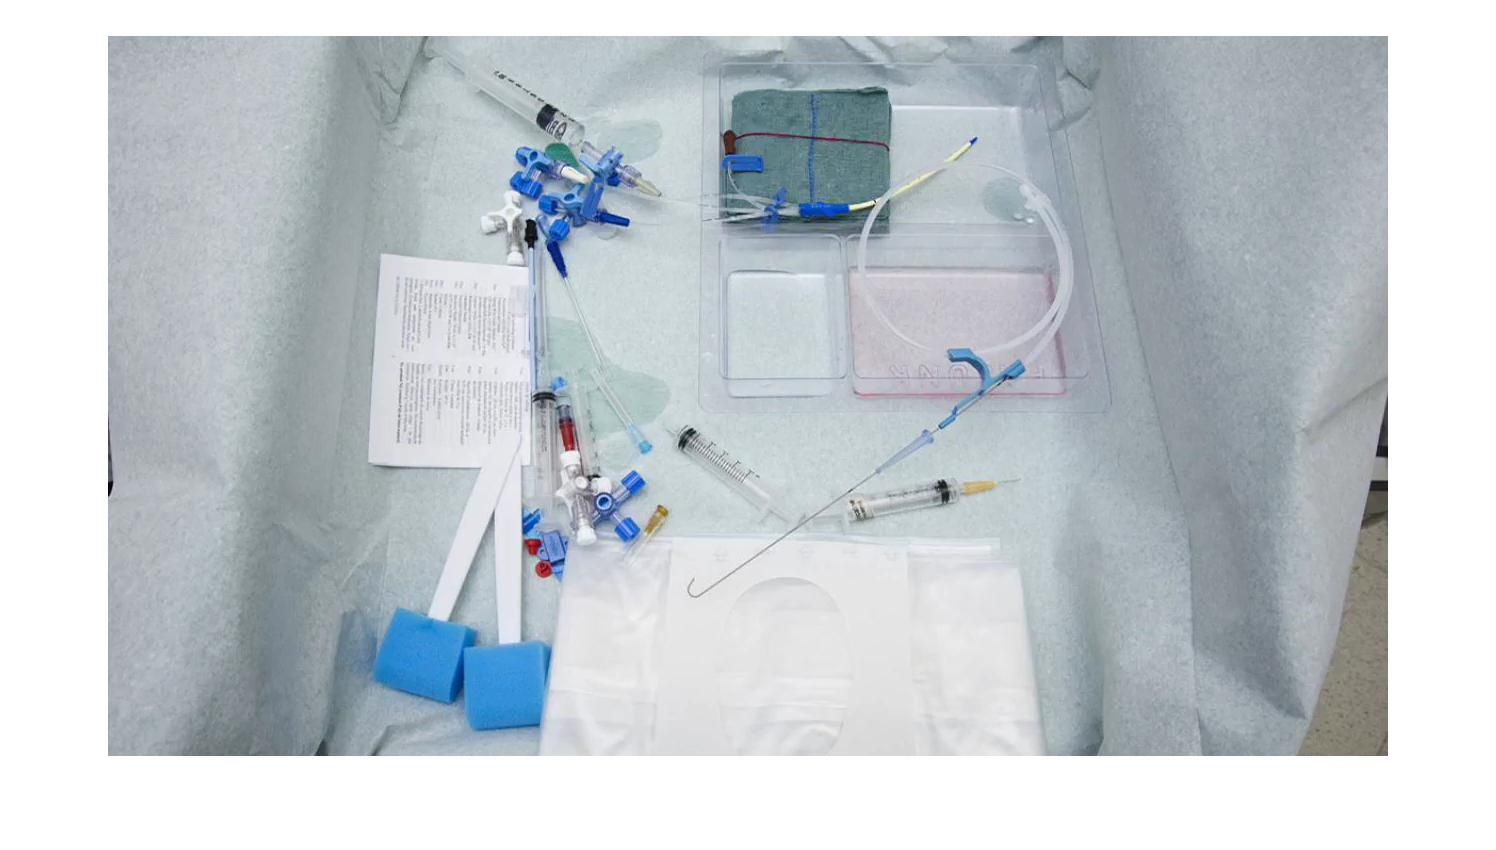
\includegraphics[width=10cm]{clip1.jpg}
				\centering
				\caption{A surgical equipment tray, with spillage under the needle}
			\end{figure}
			The data collection from the previous research project was based around a supervised eye tracking experiment in which a mixture of Expert and non-Expert Anaesthetists were asked to view a sequence of videos. These videos each depicted a scenario common to the practise, viewing an ECG screen, a surgical equipment tray etc., with a noticeable medical error in each. The subjects were prompted at the beginning of the exercise to look for these errors.
			
			During the project previously carried out by the author, the gaze data was preprocessed, filtering out variables that did not seem relevant to this problem, these were measurements taken by the Tobii camera and didn't serve a purpose for observing the subjects gaze. The resolution of the gaze data was also scaled to fit the background image for visualisation.
			
	\chapter{Approach}\label{approach}
		The solution for this problem documented in this report focuses on feature extraction from the Tobii gaze data files. These features are then reduced in dimensionality into a linear combination that helped visualise any distinction between the two groups.
		\section{Data Preprocessing}\label{datapreproc}
			Gaze data files as recorded from the Tobii eye machine come in a particular format. The machine provides a large amount of information, most of which was not used in this project. As a result the data was preprocessed before even clustering took place in order to make the information more readable for debugging. The Tobii camera gives readings for the following:
			\begin{multicols}{2}
				\begin{itemize}
					\item{Timestamp}
					\item{Number}
					\item{GazepointX (L)}
					\item{GazepointY (L)}
					\item{CamX (L)}
					\item{CamY (L)}
					\item{Distance (L)}
					\item{Pupil (L)}
					\item{Validity (L)}
					\item{GazepointX (R)}
					\item{GazepointY (R)}
					\item{CamX (R)}
					\item{CamY (R)}
					\item{Distance (R)}
					\item{Pupil (R)}
					\item{Validity (R)}
				\end{itemize}
			\end{multicols}
			Of these, only Gazepoints L and R, Timestamp and Number were used for the purposes of this project. Timestamp and number determine the time and frame of occurrence of the gaze point, whilst averages of the left and right gazepoints are taken to acquire the centre-point of focus. This results in a conversion from a table of 16 measurements to a set of X and Y value pairs. 
			
			The exercise originally contains all videos in sequence as one long video. By counting the frame index at which each clip starts within the video. These were then converted to the starting time in seconds. All timestamps are then collected into an array which is used to filter out the subset of coordinates that is relevant to the current clip. Finally, the resolution the data was recorded in by the Tobii camera is 1280x1024, whereas the first 6 clips showing images are 1280x720, and the last 8 showing videos of ECGs are 720x368. Therefore, before overlaying the gazepoints, in the tracking overlay or during clustering, the gaze data must be scaled down appropriately.
			
			Finally, the framerate of each video has been upsampled to fit the framerate of the Tobii machine, the gaze data is not affected therefore no information is lost. The only function of this is for data visualisation.
		\section{Data Visualisation}\label{datavis}
			\subsection{Eye tracking overlay}\label{overlay}
				\begin{figure}[h]
					\includegraphics[width=8cm]{eyeoverlay}
					\centering
					\caption{The first clip from the video, with the left (red), right (blue) and centre(black) gaze points of an expert}
				\end{figure}
				It seemed best to visualise the data first, in the hopes that a difference in the subjects' viewing habits would be made plain. By overlaying the gaze data per frame of the eye tracking file on the corresponding frame of the video, it was possible to follow the subjects gaze and by comparing and contrasting subjects for different clips, any difference in viewing behaviour should become plain. 
				
				This view of the data was important as early on, it was intended for a Hidden Markov Model to be fitted to each clip so that given a model for the clip it would be possible to separate any outliers, subjects who didn't behave as expected by the model, into a separate class from those who did. This did not prove viable as from the videos it was clear that while experts may spend the same time in certain areas of the screen, they did not visit each area in the same sequence, a characteristic necessary to HMMs.
			\subsection{Gaze Data Clustering}\label{datavisclustering}
				\begin{figure}[h]
					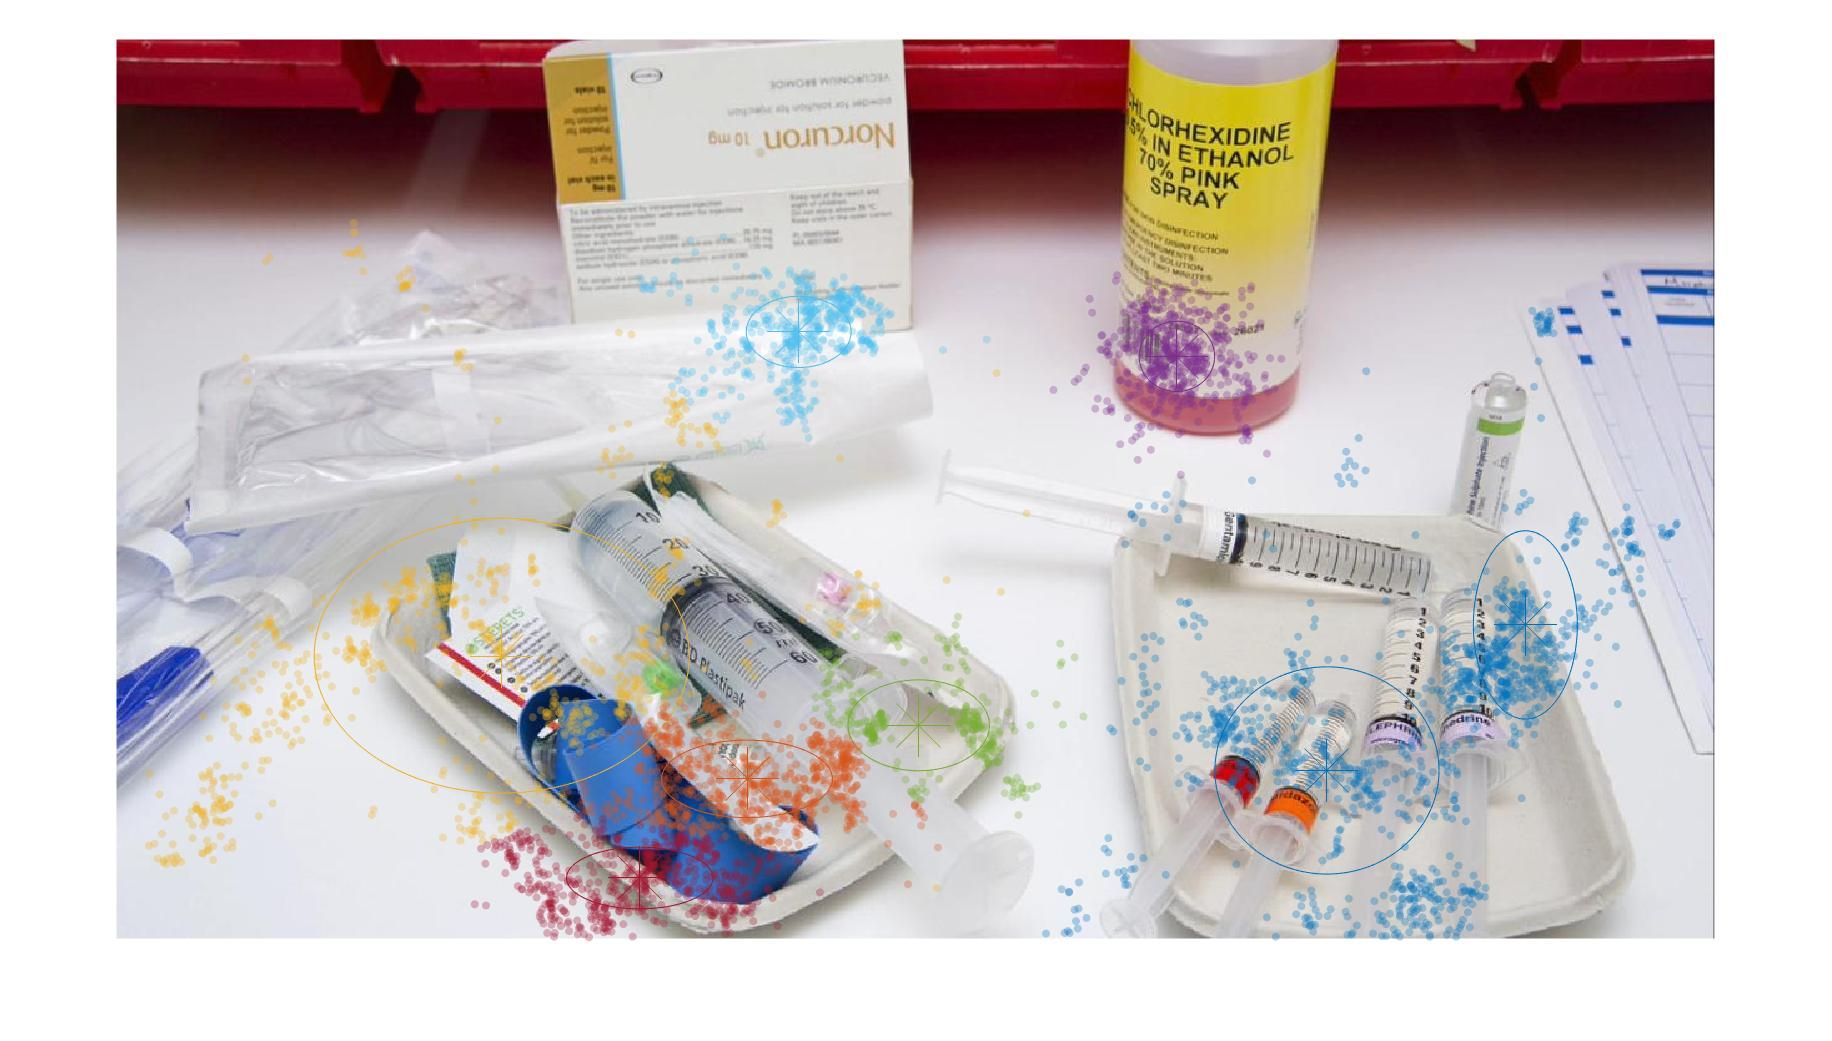
\includegraphics[width=10cm]{expertcluster}
					\centering
					\caption{Here the eye tracking data for all experts as they viewed the 3\textsuperscript{rd} clip is clustered using GMMs}
				\end{figure}
				A second approach was to cluster the gaze data of one group together over all the clip on to a freeze frame of the clip. Since the first 6 clips within the exercise video were scenes displayed in static images, the background was not temporally significant, and subjects from the same group could be compared together in order to create a heat map of sorts. For clustering, the k-means clustering algorithm was originally used. However, the clusters would often overlap or envelop smaller clusters entirely. k-Means clustering works by fitting the n observations into k sets \(S = \{S_{1},S_{2}, ..., S_{k}\}\), then minimising the variance per set\cite{kmeans}.
				
				The relatively poor clustering can be attributed to the k-means algorithm, due to its unsuitability for this data, as clusters in the gaze data are rarely circular. A different technique of clustering using a Gaussian Mixture model was much more suited as, rather than a hard border being fitted to each cluster, it instead fits a gaussian blob\cite{gmms}. The implementation first fits cluster centres using the k-Means algorithm, but then assigns data to gaussians centred around these points. By measuring the posterior probability of a gaze point belonging to each of the Gaussians in the model, a membership to that Gaussian could be assigned to that point. This accounts for points that are on the margin of two clusters for example.
				
				A GMM was then fitted to a groups data for each clip, resulting in 28 models. One requirement of clustering is to provide the number of centres to be fitted to the data. This could quite easily make the difference between good and bad clustering as assigning an incorrect number of centres could lead to two clusters being misidentified as one, or one gaussian enveloping all other data and containing any points too far from other centres to be considered as part of them, for example. However, rather than specify the number of centres based on how many clusters could be identified individually in each of 28 images, it was easier to implement a heuristic using the elbow method by incrementally increasing the number of centres, measuring the percentage of variance explained and defining a cutoff point where the gradient suddenly decreases (giving the appearance of an elbow in the graph. Percentage of variance explained is defined as the ratio of between-cluster variance to overall variance.
				
				One significant drawback with this approach to the data visualisation however, was that 7 of the 14 clips were video clips, featuring temporally dynamic stimuli, in the form of waveforms on an ECG. As the point of focus would likely move with the stimuli, removing the temporal aspect from the data would result in clusters that spanned the length of the waveform section on the screen, giving little insight into focus in a spatial respect around the crest of the wave.
				\begin{figure}[h]
					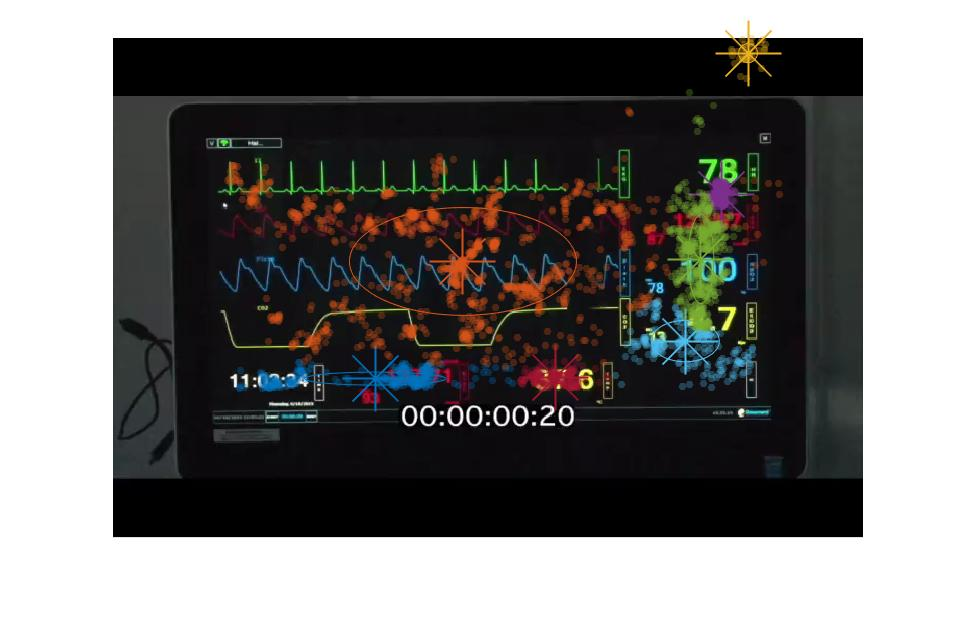
\includegraphics[width=10cm]{videocluster}
					\centering
					\caption{Poor clustering in the clip 7 due to objects moving along the screen}
				\end{figure}
		\newpage
		\section{Feature Extraction}\label{ftextrac}
			Classification on the raw gaze data alone is implausible. This is because both groups would visit the same areas in the image, quite possibly at the same time, as all stimuli in the image do not require any expertise to notice. Rather, it is in understanding them the distinction between groups would lie. Practically this means on a two dimensional space (the eye tracking data) both groups would be indiscriminable, making the task of finding a hyperplane between them meaningless. However, so long as behaviour of subjects sharing a group is similar, and as a whole different from subjects in the other group, feature extraction should provide significantly separable groups of subjects, matching their class.
			
			Also while an experts activity over the whole clip might not be meaningful enough for classification, how their activity changes over the duration of the clip could prove significant. For instance, given an experts likely familiarity with the scenes displayed in the exercise, it is logical to assume that they are able to process the apparent information faster, and they might quickly scan the clip and then rest for the remainder of the clip. For this reason each features was measured 15 times over each clip, once per second.
			\subsection{Definition of a fixation}\label{fixationdef}
				Many of the features defined in this project are statistics concerning the subjects behaviour while fixating. The definition of a fixation used for this purpose follows an algorithm defined in a paper on user attention\cite{overtva}:
				\begin{enumerate}
					\item{Calculate point-to-point velocity for each sample: }
					\item{Label each sample below 25$^{\circ}$/s as belonging to a potential fixation period, otherwise as to a saccade period.}
					\item{Merge consecutive potential fixation period samples into a fixation group, removing saccade samples. The length of these groups, or in other words the fixation duration, must be higher than 100ms. Under this threshold, the samples belonging to either a saccade or short fixation group, are discarded;}
					\item{Compute the spatial coordinates of each visual fixation (as the gravity centre of the coordinates of the samples in the considered group).}
				\end{enumerate}
				This algorithm was nicely translatable into the projects application, with a few approximations. Firstly, to measure 100ms, it was necessary to calculate the framerate of the Tobii camera, and then the number of frames recorded by the camera in 100ms. The framerate can be calculated using the total number of frames of eye tracking data \(N_{F}\) for one subjects exercise, divided by the time elapsed in seconds during the exercise, \(T\).
				\[\frac{N_{F}}{T} = \frac{16073}{320.362s} \approx 50s^{-1}\]
				At 50fps, 5 frames will transpire in 100ms. The algorithm was modified to include this, i.e. a group of potential fixations must last longer than 5 frames. 
				
				The second step was to calculate movements under 25$^{\circ}$/s. Using trigonometry to calculate the number of pixels per degree, made this a matter of conversion. The physical size of a pixel depends on what's known as the Dots per inch, or DPI of a screen. Monitors fall into categories for DPI, which are easily available online \footnote[1]{https://snapshop.cam/dpi/}. Estimating the size of the monitor used, and with knowledge that it was standard issue IT equipment for hospital staff, it seemed reasonable to settle on 72DPI, a figure confirmed by medical supervisor Dr. Lim. By making approximations of the distance the viewer sat from the screen, and assuming a sitting distance of 45cm, or 17.71654in the distance travelled by the gaze in pixels as a result of turning the eye 25$^{\circ}$ is:
				\[d_{px} = \lvert{\frac{17.71654 tan(25)}{72}}\rvert \approx 170.32px\]
				Therefore, \(1^{\circ} = \frac{170.32}{25} \approx 7px\).
			
				For features that used the cluster of the gaze point, it was also necessary in the algorithm for a fixation to remain in the same cluster for it's duration.
				
			\subsection{Assigning clusters}\label{choosingcluster}
				When assigning each data point to a cluster, the expert model was used for each clip. The expert clustered much more nicely, and better defined the objects in the scene. This also suited a larger decision made whilst designing the classifier \ref{classification}.
				\begin{figure}[h]
					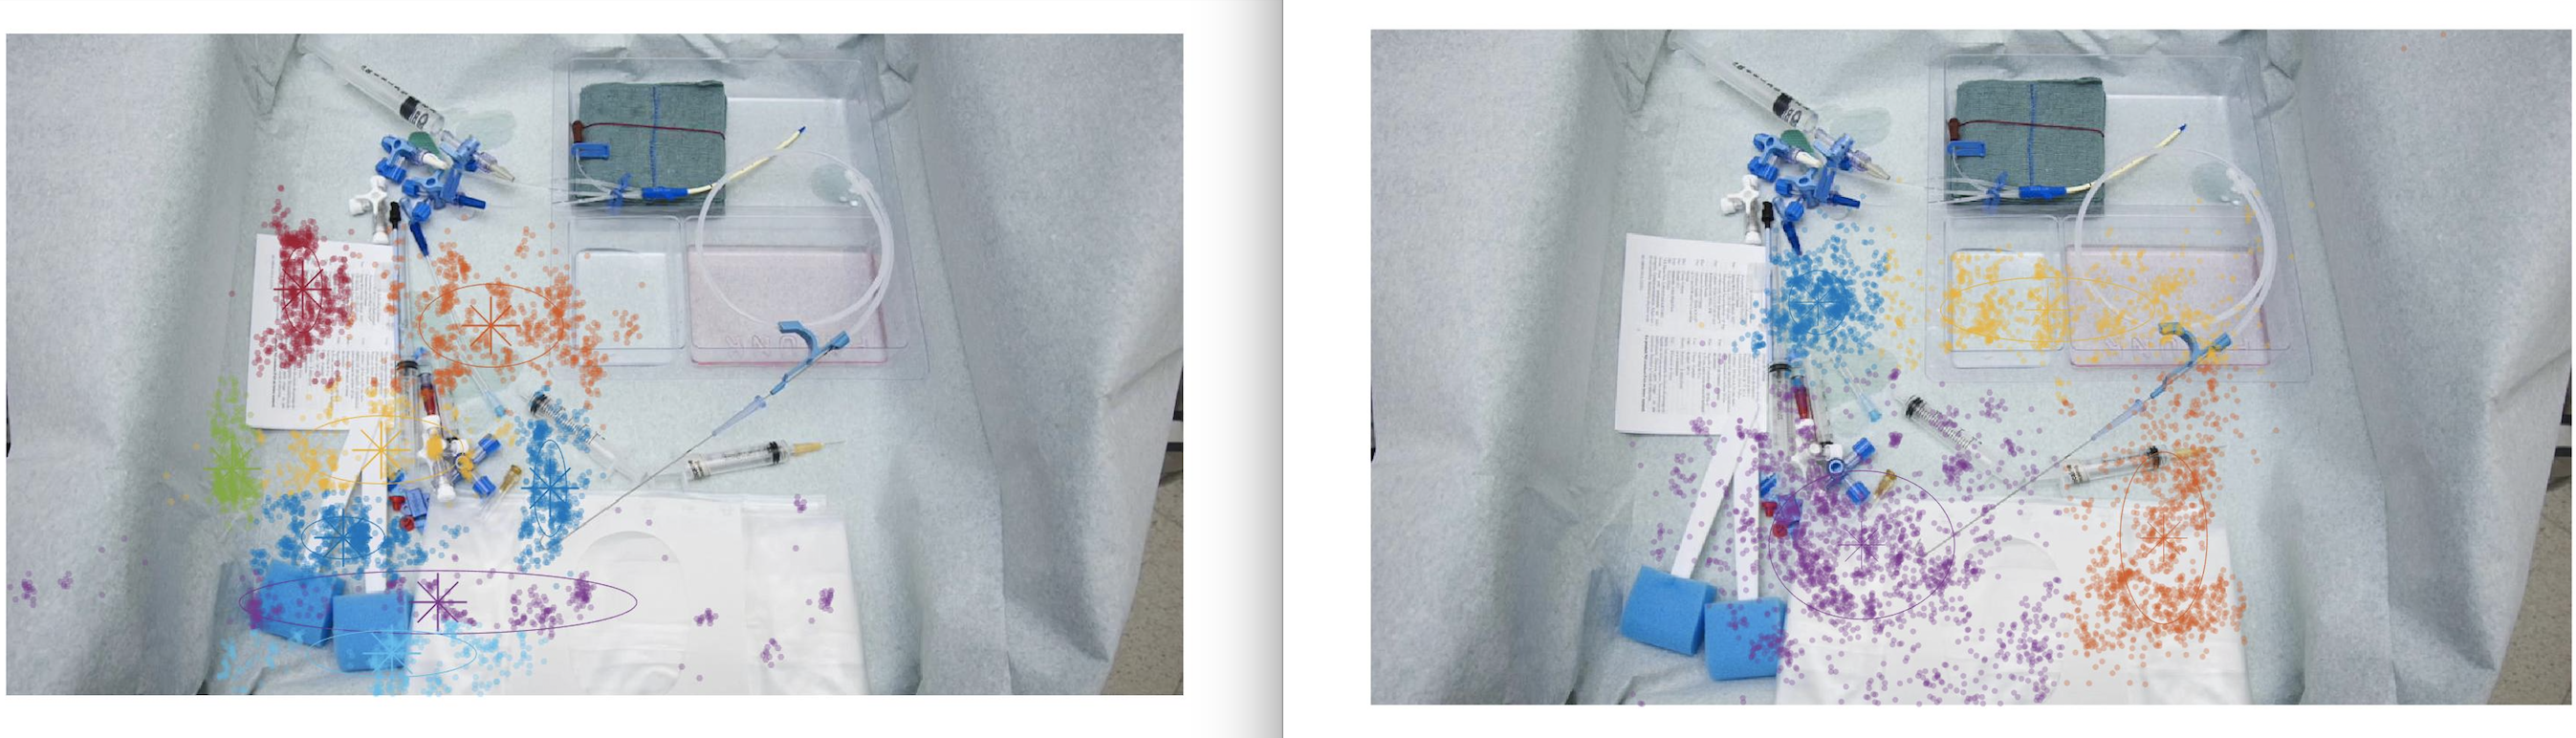
\includegraphics[width=12cm]{clustercomparison}
					\centering
					\caption{A side-by-side comparison of the clustering of expert (right) and lay (left) data shows that expert clusters span much more of the screen and demarcate well defined regions within the scene, whereas lays only cover one half of the screen}
				\end{figure}
				
			\subsection{Spatial features}\label{spatialft}
				Spatial features are measures of how the subject moves around the screen, for example the distance travelled in the exercise by the gaze around the screen.
				
				From the overlaid eye tracking clips it appeared that Experts were more steady in their gaze, and defined a smoother path, travelling back on themselves less than the Lays seemed to. Such a distinction would make itself clear in spatial measures of the gaze data. Therefore, the mean variance within a cluster for each second long section of the clip is used. 
				
				Lays on the other hand appeared to travel quite erratically from point to point, regularly flicking back to previously visited areas and apparently losing attention much more frequently. Such behaviour would manifest itself as a huge difference in distance travelled, defining a second spatial feature.
				
				Another hypothesis that experts might accelerate more rapidly towards each cluster, as they recognised and honed in on the stimuli at the center of that cluster is also tested.
				
				As another feature, the total number of transitions made from one cluster to another is used, to which the observation of lays flicking between regions frequently lends confidence to.
				
				In summary, four spatial features were measured 15 times over a 15 second duration:
				\begin{itemize}
					\item{Average in-cluster variance.}
					\item{Total distance travelled by gaze.}
					\item{Average acceleration towards a cluster.}
					\item{Total transitions from one cluster to a different cluster.}
				\end{itemize}
			\subsection{Temporal Features}\label{temporalft}
				Temporal features would describe the how subjects spend their time during the exercise, i.e. how long they focus on any particular thing, or how often they focus.
				\subsubsection{Cluster Features}\label{temporalcluster}
					Following the same logic used for Spatial features, it would stand that Experts would spend less time focusing on any area as they should recognise errors quickly from experience and training. This was translated to average duration spent in one cluster. However, as some of the clusters are quite large, with some covering around 30-40\% of the screen, it is possible that the gaze could remain in one cluster for an extended period of time without fixating for the most of that time. So the total number of fixations in a cluster was taken as an additional measure.
				\subsubsection{Non-Cluster Features}\label{temporalnoncluster}
					In order to account for unsuccessful clustering, as in the ECG clips, and behaviour that might not remain within a cluster, or where the cluster is not significant, it was also important to take a selection of temporal features that do not consider the cluster data, rather just measuring features from the raw gaze data.
					
					Time taken before the subject fixates at the very beginning of the clip was used to measure how quickly experts find and focuses on an object in the scene.
					
					The total number of fixations and the average duration of a fixation per section also seemed promising, based on the observation that Experts seem to hone in on objects and remain for longer, i.e. fixating less frequently and for longer. Similar to these features, is the time spent not fixating, with the hypothesis that Lays would spend more time scanning rapidly across the scene.
				\\
				\\
				In summary six suitable temporal features were found, again measured 15 times during the clip, excluding time to initial fixation, which was measured only once:
				\begin{itemize}
					\item{Cluster features}
					\begin{itemize}
						\item{Average in-cluster duration.}
						\item{Total number of in-cluster fixations.}
					\end{itemize}
					\item{Non-cluster features}
					\begin{itemize}
						\item{Time until initial fixation.}
						\item{Total number of fixations.}
						\item{Average duration of a fixation.}
						\item{Time spent not fixating.}
					\end{itemize}
				\end{itemize}
		\newpage
		\section{Dimensionality Reduction}\label{dimensionalityreduc}
			With 10 total potential features, with each feature measured and recorded 15 times per clip, classification would be in 150$^{th}$-dimensional space. This would then be increased considerably by the SVM as the purpose of the kernel trick is to increase dimensionality of the data to find hidden separation (explained in \ref{bgsvms}).
			
			Therefore, although compiling a large number of features would increase the likelihood of finding a distinguishing relationship between the groups, it also increases the complexity of training and testing the resulting classification model. When implementing dimensionality reduction, using the correct method should reduce the complexity of the data with minimal loss of information. Two popular methods that provide additional advantages have been chosen.
			\subsection{t-SNE}\label{drtsne}
				t-distributed Stochastic neighbour embedding is a non-linear dimensionality reduction method\cite{tsne}. In two stages, it fits a probability distribution to pairs of points in the high dimensional data such that similar points have a high probability, and that conversely dissimilar points have very low probability. A p.d. is then defined with lower (2\textsuperscript{nd} or 3\textsuperscript{rd}) dimensionality. The divergence of these p.d.s is then reduced such that similar points in the high dimensional data have mappings with similar probability in the lower dimensional representation. This method is particularly useful for data visualisation, as relationships between data are preserved in a visualisable dimension. However information isn't technically retained, as the probability distribution of similarity between points does not account for magnitude for instance. t-SNE can be performed using a variety of distance metrics, of which Cosine, Euclidean and Chebychev distance were used, for comparison. A fourth measure, Mahalanobis distance was not possible with this data as it requires that the covariance of the data be symmetric.
			\subsection{PCA}\label{drpca}
				Principal Component Analysis is a linear dimensionality reduction method, for data with multiple correlating dependent variables. In short, PCA transforms the data onto a new coordinate system that emphasises patterns and variance in the data\cite{pca}. It does this by projecting the data onto the new coordinate system such that the most variance in the data is on the first axis, the next most on the second and so on. Intuitively, in a coordinate system where variance in the data is at it's most, finding separation between subsets of the data will be at it's easiest. It is for this reason that PCA lends very strongly to classification methods that separate the data, notably SVMs. As each of the new coordinates, or principal components, is a linear combination of the original axes, the dimensionality of the data is also reduced. As the principal components are sorted in order of decreasing variance, by definition, selecting the first n principal components such that these account for more than say 90\% variance, means that any additional principal components can be discarded with only 10\% variance lost. This cutoff can be tweaked as appropriate, or can suit the number of desired dimensions. However, data that is evenly spread, for instance circular, will result in relatively even distribution of variance between principal components resulting. In this scenario the resulting loss in variance would be significant enough for dimensionality reduction to be much less feasible. Two matrices are conventionally outputted as a result of the PCA algorithm, the first, a set of coefficients or loadings, containing rows of coefficients for each column relating to a principal component. The loadings allow by matrix multiplication the conversion of data from the original feature space into principal component space. The second matrix is the converted data used to find the components.
				
				In this project, PCA proved very effective not only for visualising relationships between data in a lower dimensionality, but also effectively providing a linear combination of the most distinguishing variables of data, along with a relatively simple means of converting any new data into this format.
		\section{Classification}\label{classification}
			Classification is the main objective of this project. There are various approaches that can be taken to classification in order to to fully assess the plausibility of classifying expert and non-expert. Given 150 variables, it is simple single variable classification as well as evaluate pairs of variables for classification. 
			\subsection{Single-variable and pairwise classification}\label{singleandpair}
				Classifying using a single variable is a simple method for assessing that variables usefulness in the model. Since the dimensionality is as low as it can be and no preprocessing need occur before classification, it is prudent to test each variable. Secondly, by creating a heat-map of variables classified in pairs, weak and strong areas in classification could be visualised.
			\subsection{Sequential Forward Selection}\label{sequentialforwardselec}
				A popular search method in feature space known as sequential forward selection is a useful heuristic for building an effective classification model. Sequential forward selection adds features from the feature space sequentially until the loss, which can be user defined, increases. The main drawback of this technique is that if poor features are ordered first, these will be added, increasing the loss, and therefore ending the process before better features can be added\cite{sfs}. Sequential feature selection becomes considerably more practical a method once the variables are sorted in order of descending accuracy. Effectively allowing SFS to create a partition of useful and non-useful variables, where usefulness is determined by contribution to the classification models accuracy. A counterpart of SFS is sequential backward selection, which begins with a model including all variables, and incrementally removes them until the accuracy decreases.
			\subsection{Classification in Principal Component space}\label{classifyingpca}
				As previously explained PCA is very useful for maximising the variance in the data. It is as a result of PCA that the potential separation between experts and non-experts in feature space is most defined, this should make the SVMs job considerably easier if in the original feature space separation is very slight.
			\subsection{Fine tuning parameters}\label{finetuningsvm}
				There are many parameters in a SVM model that can be tweaked to better fit the scenario. The strongest and most apparent example being the kernel function used to transform the data into a higher dimensional space. There are three built-in functions available, namely linear, gaussian or radial basis function and polynomial kernels. Each function is suited to a different application. For instance, the gaussian kernel is default for one-class learning \cite{oneclasswgaussian}. The polynomial kernel is used in cases where data is not linearly separable in feature space but requires the order of polynomial used to be provided.
				
	\chapter{Implementation}\label{implementation}
		This chapter documents the resources, libraries and implementation used to achieve the methods listed in approach.
		\section{Environment}\label{devenv}
			This project was carried out entirely within software and a development environment. As data was gathered as part of a previous project, there was no need in this project for crafting the viewing exercise or carrying it out on subjects. As a result the ethics of the data did not come into question.
			\subsection{MATLAB}\label{matlab}
				Matlab is a programming language tuned towards mathematical and scientific programs developed by Mathworks. With heavy focus on mathematical formula and data visualisation it is a very popular tool for data scientists and analysts. The development environment provides an intuitive means of debugging code. Matlab provides a variety of licensed toolboxes for additional functionality such as Machine Learning and Image Processing. As a result, the Matlab community has a heavy focus on scientists and academics, providing a lot of support in the scope that this project falls in. This all makes Matlab an excellent choice for this project as with the aforementioned Machine Learning Toolbox, along with various other external toolboxes and libraries provided by the community, the main goal of the project could be focused on with very little distraction in terms of ancillary functionality that would otherwise reduce the time available to carry out the necessary experiments documented in \ref{approach}.
		\section{Toolboxes and Libraries}\label{toolbox}
			Many algorithms and methods necessary to the project approach have already been implemented, either officially by Mathworks or by the Matlab community. Implementations of clustering methods and dimensionality reduction for instance are outsourced in this project to available toolboxes.
			\subsection{Statistics and Machine Learning Toolbox}\label{statsandml}
				This official Matlab toolbox was essential for this projects success. Providing not only highly customisable methods for classification, but also clustering, data partitioning and dimensionality reduction.
				\subsubsection{Clustering}\label{statsandmlclustering}
					The function used for \texttt{kmeans} clustering can be found in this toolbox. The \texttt{kmeans} function takes as it's mandatory arguments the data in a matrix X of n observations of p variables, and k, the number of partitions into which X is split by the algorithm. As the clustering method was later changed to GMMs \ref{datavisclustering} the k-means method is not used in the final implementation of the solution.
				\subsubsection{Dimensionality Reduction}\label{statsandmldr}
					Implementations of both t-SNE and PCA are both available through the Stats and ML toolbox. The \texttt{pca} function takes a matrix X of n observations of p variables, and outputs 3 notable values. The loadings matrix \texttt{coeff}, the principal component scores in \texttt{score}, and \texttt{latent}, a vector of the explained variability of each principal component. 
					
					As mentioned before in \ref{drtsne}, t-SNE can be used for data visualisation. The function \texttt{tsne} takes as its arguments, the matrix X, in the same format as \texttt{pca} and \texttt{kmeans}. It can also take Name-Value pairs, including 'Distance' followed by 'mahalanobis', 'cosine', 'chebychev' or 'euclidean'. Another notable optional parameter is 'NumDimensions' which is by default 2, but can also be 3 for 3 dimensional data representation.
				\subsubsection{Classification}\label{statsandmlclassification}
					The main and final goal of this project is successful classification of experts and non-experts. The Stats and ML toolbox provides a ClassificationSVM class, with methods for fitting, \texttt{fitcsvm}, and predicting, \texttt{predict}, a SVM model. There are also methods for cross evaluation, \texttt{crossval}, and finding the estimated loss of the model, \texttt{kfoldLoss}.
			\subsection{NETLAB}\label{netlab}
				The NETLAB toolbox provides various functionality for pattern recognition. It was suggested for the project as a solution to the poor clustering provided by the k-means algorithm as it contains an implementation of Gaussian Mixture models for clustering data. The GMM code consists of several functions (gmminit, gmmpost etc.) that allow the creation, initialisation, fitting and EM training of a GMM. These were possibly the most used out of all methods used for data preprocessing and analysis, being at least on par with the SVM methods for use. In the NETLAB implementation, a GMM is created with the function gmm, taking parameters for number of dimensions, number of centres and type of covariance matrix. The model can then be initialised on a data set using gmminit before finally being run through the Expectation Maximisation, or EM algorithm to fit the model to the data.
			\section{Algorithms}
				This section documents the implementation in Matlab of some of the algorithms listed in \ref{approach}.
				\subsection{Data Preprocessing}
					While this code was developed as part of the previous project in preprocessing the gaze data, it is noteworthy as it scales and filters the gaze data from its raw format.
					\newpage
					\lstinputlisting[caption = {This code filters out data for the specific clip, using an array of timestamps, and the clip no. taken as an argument. It then scales the resolution down depending on the clip.}]{scaledata.m}
				\subsection{Data Visualisation}
					\subsubsection{Overlay}
						In order to visualise the tracking data overlaid on the background clip, an algorithm that would plot the data as points, on the same figure as the image, for each frame was necessary. In order to better visualise the movement, a line between the previous and current gaze points is plotted, giving the appearance of gazepoints leaving a short trail as they move. 
						\newpage
						\lstinputlisting[caption = {This code provided the initial data visualisation necessary to disproving the feasibility of using HMMs \ref{datavis}}]{overlay.m}
					\subsubsection{Clustering}
						The final incarnation of the clustering algorithm used in this solution is a combination of clustering using GMMs repeatedly, incrementing the number of centres, until the rate of change of explained variance per cluster decreases past a cutoff point, in what's known as the elbow method. The implementation of which is featured below.
						\lstinputlisting[caption = {Here, the number of gaussians is increased every iteration until the error of the GM model increases by at least 1}]{elbowmethod.m}
Results and Evaluation
				\subsection{Classification}
					\subsubsection{Classification on a single variable}
						By evaluating each variables independent performance, not only is that variables usefulness in the end model but also aided the sequential forward selection approach as variables could be sorted in descending order of accuracy.
						\lstinputlisting[caption = {Each variable, represented by a column of the data, is used to fit a 1 dimensional SVM, which is then cross validated, and the loss for that model estimated}]{singleft.m}
	classification on features as a whole
	pairwise classification
	sequential feature selection
	classification after pca
	classification on interpolated pca data with tuned parameters
	
	
Conclusions + Future Work
	talk about generalisation of expert classification
	
Reflection on Learning
Glossary
Table of Abbreviations - optional
Appendices
	\begin{thebibliography}{2}
	\bibitem{eyemovements}
	Purves D, Augustine GJ, Fitzpatrick D, et al., (2001)
	\textit{Types of Eye Movements and Their Functions 2\textsuperscript{nd} edition}
	Sunderland (MA): Sinauer Associates.
	\texttt{https://www.ncbi.nlm.nih.gov/books/NBK10991/}
	\bibitem{vapnik-svms}
	Cortes C., Vapnik V., (1995)
	\textit{Support-vector networks}
	Machine Learning 20(3),
	Springer
	\bibitem{overtva}
	O. Le Meur, et al., (2010)
	\textit{Overt visual attention for free-viewing and quality assessment tasks Impact of the regions of interest on a video quality metric}
	Elsevier
	\bibitem{kmeans}
	Lloyd, S. P. (1957)
	\textit{Least square quantization in PCM}
	Bell Telephone Laboratories Paper. 
	Published in journal much later: Lloyd., S. P. (1982).
	\bibitem{gmms}
	Nabney, I. T., (2004)
	\textit{NETLAB: Algorithms for Pattern Recognition}
	Springer, ch. 3
	\bibitem{tsne}
	van der Maaten L., Hinton G., (2008)
	\textit{Visualising Data using t-SNE}
	Journal of Machine Learning Research 9 2579-2605
	\bibitem{pca}
	Abdi H., Williams L. J., (2010)
	\textit{Principal Component Analysis}
	WIREs Comp Stat, 2: 433-459. 
	\bibitem{sfs}
	Marcano-Cede�o A., Quintanilla-Dom�nguez J., Cortina-Januchs M.G., Andina D., (2010)
	\textit{Feature selection using Sequential Forward Selection and classification applying Artificial Metaplasticity Neural Network}
	IEEE
	\bibitem{oneclasswgaussian}
	Chen Y. Q., Zhou X., Huang T. S., (2001)
	\textit{One-class SVM for learning in Image Retrieval}
	IEEE Conference on Image Processing
	\end{thebibliography}
\end{document}
